\subsection{Opgave 49}

På figuren ses grafen for funktionen f.

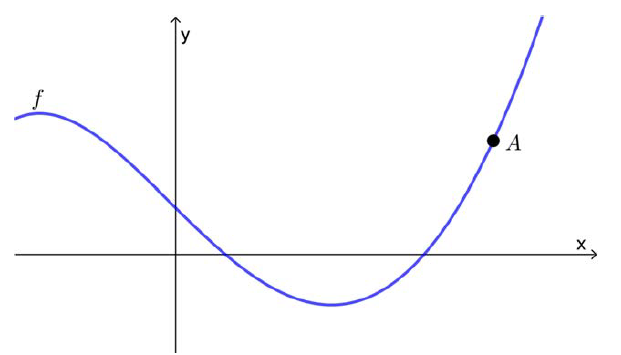
\includegraphics[width=8cm]{Opgave_41-50/Opgave_49/49.png}

Tegn både en sekant og en tangent gennem punkt A.

\ans

En tangent igennem et punkt er en ret linje som går igennem punktet og følger hældningen på funktionen i punket.

En sekant igennem et punkt er en ret linje som går igennem punktet og 1 andet vilkårligt punkt på grafen.

Nedenfor er tangenten indtegnet som den røde linje og sekanten indtegner som den sorte linje.

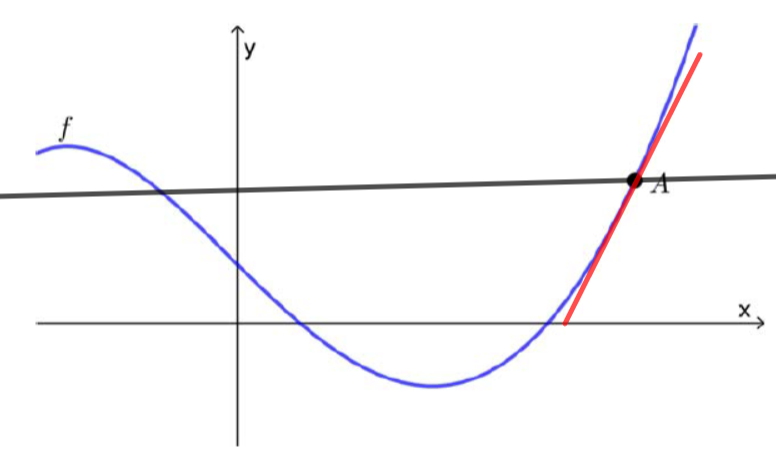
\includegraphics[width=8cm]{Opgave_41-50/Opgave_49/49.1.png}

